\newpage
\section{FUTURE SYSTEM ENHANCEMENT}

                     \subsection{Feature Extraction}
                     Most of the job in this part has been completed. Some of the remaining tasks are:
                     \begin{enumerate}
                             \item Extracting the Pitch Feature. It will be the foremost job for this section of the project in the coming days. 
                             \item Optimizing the extraction process and making it faster and less memory extensive.
                             \item Initial tinkering with the weights have shown that Intensity is highly influential in the clustering process and that the other two features aren't contributing much to the results. This will be investigated.
                             \item The role and affect of the various constants and assumptions used during feature extraction will be analyzed. 
                             \item Code Refactoring and Documentation.
                     \end{enumerate}

                     \subsection{K-means Clustering}
                     The basic implementation has been completed. Other work in this area will be to extend it:
                     \begin{enumerate}
                             \item Trying out different initialization methods discussed in [4] and studying their effects.
                             \item Trying out different distance metrics and studying their effects.
                             \item Investigating why the accuracy is poor for genre other than Hiphop.
                             \item Using measures for cluster quality such as Entropy, Purity, etc. 
                             \item Code Refactoring and Documentation
                     \end{enumerate}

                     \subsection{Artificial Neural Network and Mood Based Classification}
                     Nothing has been done in this part of the project. So, it will take up the majority of the efforts in the coming days:
                     \begin{enumerate}
                             \item Research
                             \item Code Implementation
                             \item Training set collection
                             \item Validation methodologies determination
                     \end{enumerate}

                     \subsection{Application Development}
                     The project aims to develop an application with following features:
                     \begin{enumerate}
                             \item Ability to list out all mp3 fles on the accessible File-system. 
                             \item Basic media player abilities: play, pause, stop, previous, next. 
                             \item Create smart playlists: \\
                                      - Playlists with similar songs\\ 
                                      - Playlists that focus on variety \\
                                      - Playlists that interpolate/add songs between any two given songs
                     \end{enumerate}
                     Developing this application will also take up a lot of the time and effort.
                     \newpage
                     \subsection{Gantt Chart}
                     The gantt chart for the remaining task is as:
                     \begin{figure}[h]
                             \centering
                             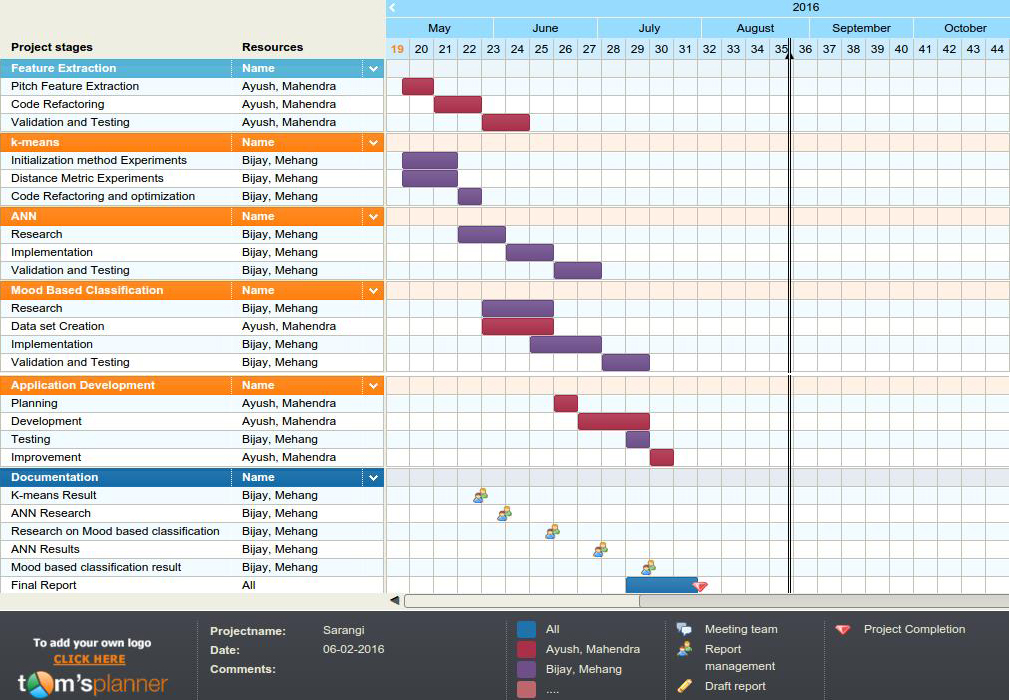
\includegraphics[width=170mm]{resources/ganttchart.jpg}
                             \caption{Gantt chart for the remaining task}
                             \label{fig:figure 11}
                     \end{figure}
